\documentclass[a4j,9pt,twocolumn,dvipdfmx]{jsarticle}
\usepackage{apulayout}

\begin{document}
\mktitlem{修士論文タイトル}
{県大 太郎}{情報 花子}

\section{はじめに}
この文書では，愛知県立大学大学院~情報科学研究科の修士論文の要旨
（以降，要旨）の共通レイアウトの利用について説明しています．この文書にあ
る説明を参考にして要旨を作成して下さい．

\section{ドキュメントクラスの指定}
要旨は日本語で作成するので \LaTeX のドキュメントクラスは
\texttt{jsarticle} を使用します．オプションには，用紙サイズ \texttt{a4j}，
フォントサイズは$9$，または$10\ {\rm pt}$を指定して下さい．
また，要旨は二段組で作成するので \texttt{twocolumn} も指定して下さい．
要旨はPDFファイルで提出するため，\texttt{pdfdvimx}を使うことになると思われますので，
ドキュメントクラスのオプションとして指定しておきます．
\begin{screen}
 \begin{small}
  \verb#\documentclass[a4j,9pt,twocolumn,dvipdfmx]{jsarticle}#%
 \end{small}
\end{screen}

\section{レイアウト設定用ファイルの読み込み}
この文書と一緒に配布されている \texttt{apulayout.sty} をドキュメントクラ
スの指定直後に \verb#\usepackage# コマンドで読み込んで下さい．
\begin{screen}
 \begin{small}
  \verb#\documentclass[a4j,9pt,twocolumn,dvipdfmx]{jsarticle}#\\[-0.5em]
  \verb#\usepackage{apulayout}#
 \end{small}
\end{screen}

\texttt{apulayout.sty} には，要旨のレイアウトに必要な設定，コマンドが記
述されているので変更しないように注意して下さい．

設定用ファイル中で要旨の作成に必要な基本的なパッケージの読み込みは行っ
ています．読み込み済みのパッケージは \texttt{amsmath}，\texttt{amssymb}，
\texttt{ascmac}，\texttt{graphicx} です．また，レイアウト用に
\texttt{fancyhdr}，\texttt{nidanfloat}，\texttt{geometry} パッケージの読
み込みも行っています．
このほかのパッケージが必要な場合には，\texttt{apulayout.sty} を読み込ん
だ後に，各自で読み込みを行って下さい．

\section{要旨タイトル部分}
要旨のタイトル部分は \verb#\mktitlem# コマンドを使用します．

\verb#\mktitlem# コマンドには $3$ つの引数があります．それぞれ，修士論文
タイトル，学生氏名，指導教員氏名を指定します．
\begin{screen}
 \begin{small}
  \verb#\begin{document}#\\[-0.5em]
  \verb#\mktitlem{修士論文タイトル}{学生氏名}{指導教員氏名}#
 \end{small}
\end{screen}

このコマンドは，
\texttt{document} 環境の開始直後に指定します．

\section{二段組時の特殊な図，表の配置}
要旨は二段組で作成するため，横に長い図や表を \texttt{figure} や
\texttt{table} 環境を使用して配置すると A4 用紙一枚に収まらなくなります．
その場合には \texttt{figure*} や \texttt{table*} 環境を使用して下さい．
\figurename\ref{fig:exp} や \tablename\ref{tab:exp} のように要旨の上部，
または下部に自動的に一段組で配置されます．
ただし，要旨が $2$ ページにわたる場合には，$1$ ページ目に配置される図と
文章が重なってしまいます．この場合には $1$ ページ目の途中で
\verb#\pagebreak# コマンドを使用して改ページを行って下さい．
\begin{itembox}[l]{\texttt{figure*} 環境の記述例}
 \begin{small}
  \verb#\begin{figure*}#\\[-0.5em]
  \verb# \begin{center}#\\[-0.5em]
  \verb#  \includegraphics{fig.eps}#\\[-0.5em]
  \verb# \end{center}#\\[-0.5em]
  \verb#\end{figure*}#
 \end{small}
\end{itembox}

\begin{figure*}
 \begin{center}
  \includegraphics[width=0.8\textwidth]{figsample.eps}
  \vspace{-1em}
  \caption{二段抜きの例（\texttt{figure*}環境）}
  \label{fig:exp}
 \end{center}
\end{figure*}

\begin{table*}
 \caption{二段抜きの例（\texttt{table*} 環境）}
 \label{tab:exp}
 \vspace{-1em}
 \begin{center}
  \begin{tabular}{|c|c|}
   \hline
   要素 $1$&要素 $2$\\
   \hline
   二段組では表現がし難い横に長い表も&\texttt{table*} 環境を使えば二段抜きにすることができます．\\
   \hline
  \end{tabular}
 \end{center}
\end{table*}

\section{サンプル 1}
21世紀における豊かで持続的に発展する社会を構築することは，現代の私達，人
類の共通した責務であると思います．特に，愛知県を中心とする東海地区は輸送
機械，工作機械産業を中心に，世界でも有数の先進的工業集積地です．近年機械
工業製品に関する急速な知能化の進行は，この地区の産業についても情報システ
ムを活用した付加価値の高い知識集約型産業への転換を求めています．また，高
度情報化社会への対応，自然環境の脆弱性に注目した人間活動の枠組みの決定，
高度な医療・福祉社会への対応など，地域社会は多くの問題に直面しています．
これらは，21世紀初頭までに解決の糸口を見出しておくべき課題です．

このような情勢の変化に対応するため，本学情報科学部は情報システム学科およ
び地域情報科学科との2学科構成として，平成10年4月から発足しました．情報シ
ステム学科では，最新の情報システム，マルチメディア技術に関する学術研究を
行うとともに，これを基礎にした専門的知識と技術を学生諸君に伝え，各種の情
報システムを自由に構築，運用することのできる情報システム技術者を養成しま
す．また，地域情報科学科では，情報処理技術に関連した情報ネットワーク，コ
ンピュータシミュレーションに関する学術研究を行うとともに，これを基礎にし
た専門的知識と技術を学生諸君に伝え，地域の情報化に不可欠な各種の情報ネッ
トワークと，
地域環境の分析，設計に不可欠なシミュレーションシステムを自由
に構築，運用することのできる情報システム技術者を養成します．本情報科学
部では，高等学校卒業者を対象にした一般選抜，社会人を対象にした社会人特別
選抜，職業に関する学科の高等学校出身者を対象にした推薦入学，高等専門学校
および短期大学卒業者を対象にした3年次編入学などにより，多様化した社会に
対応するため広範な入学者募集を行います．なお，本情報科学部では，平成14
年度に大学院情報科学研究科情報科学専攻修士課程を設置し，さらに，平成16年
度に大学院情報科学研究科博士課程（前，後期課程）を設置し，大学院教育を開
始しました．前期課程入学定員25名後期課程入学定員5名です．前期課程では，
ものづくりと情報技術を結合させた次代を拓く新しい情報システム技術者の養成
を目指しています．また，同後期課程では，研究者の養成も視野に入れながら，
情報システム関連分野における新技術の開発を目指した高度情報システム技術者
の養成を行うこととしています．．\hfill{\cite{www1}より転載
%\pagebreak

\section{サンプル 2}
After a seven-year journey, a NASA space capsule returned safely to
Earth on Sunday with the first dust ever fetched from a comet, a cosmic
bounty that scientists hope will yield clues to how the solar system
formed.

The capsule's blazing plunge through the atmosphere lit up parts of the
western sky as it capped a mission in which the Stardust spacecraft
swooped past a comet known as Wild 2.

Ron Ceeders, a Lockheed Martin technician, unbolts a canister containing
comet dust from the Stardust capsule in a clean room Sunday, Jan. 15,
2006, at Dugway Proving Ground, Utah. [AP]

"This is not the finish line. This is just the intermediate pit stop,"
said project manager Tom Duxbury of the Jet Propulsion Laboratory in
Pasadena, Calif., which managed the \$212 million mission.

About a million comet and interstellar dust particles --- most
smaller than the width of a human hair --- are believed to be inside
a sealed canister.

The particles are thought to be pristine leftovers from the birth of the
solar system about 4.5 billion years ago. Some samples could be even
older than the sun.

The next stop for the capsule is the Johnson Space Center in Houston,
where scientists will unlock its canister later this week. After a
preliminary examination, they will ship the particles to laboratories
all over the world for further study to analyze their composition.

"Inside this thing is our treasure," said principal mission scientist
Don Brownlee of the University of Washington.

Stardust's successful return was welcome news to the space agency, which
suffered a setback in 2004 when its Genesis space probe carrying solar
wind atoms crashed into the same Utah salt flats and cracked open after
its parachutes failed to deploy.

After the Genesis mishap, engineers rechecked Stardust's
systems. Duxbury said its return home went "like clockwork."

Early Sunday, the Stardust mothership released the shuttlecock-shaped
capsule, which plunged through the atmosphere at 29,000
mph.

The first parachute unfurled at 100,000 feet, followed by a larger
chute, which guided the capsule to a 10-mph landing at Dugway Proving
Ground. There was a tense moment in mission control when engineers could
not immediately confirm the first parachute had opened.

Before coming to rest on its side, the capsule bounced three times but
didn't crack, said Joe Vellinga of Lockheed Martin, who helped lead the
recovery.

Scientists in white protective suits spent the day cleaning the capsule
and its canister of dust samples before the trip to Johnson Space
Center. It will be days before engineers learn how well the capsule's
heat shield held up during the fiery re-entry.

The Stardust mothership remains in orbit around the sun and NASA is
considering sending it to another comet or asteroid to snap
photos. There won't be another chance for a sample return, however,
because the craft carried only one capsule.
\centerline{$\vdots$}\\[-0.5em]
\hfill{\cite{www2,www3} より転載}
\section{おわりに}
この要旨作成用のレイアウト設定ファイルの動作確認は，Vine Linux 3.2 上の
\texttt{tetex-2.0.2-0vl14} がインストールされている環境で行いました．

この文書は \LaTeX を使用して要旨を作成するときに共通のレイアウトの利用に
ついてのみ説明しています．\LaTeX の基本的な操作やコマンド，環境について
は演習室で閲覧することのできる \cite{美} や \cite{典} を参照して下さい．
また，インターネットを利用して検索することも効果的です．

\begin{thebibliography}{9}
\begin{small}
 \bibitem{美} 奥村晴彦 『\verb#[#改訂版\verb#]# \LaTeX2e 美文書作成入門』 技術
       評論社，2003
 \bibitem{典} 生田誠三 『\LaTeX2e 文典』 朝倉書店，2001
 
\bibitem{web}
	\texttt{http://pcg-xr1g.hp.infoseek.co.jp/cat\_latex.shtml}
\bibitem{www1}
	\texttt{http://www.aichi-pu.ac.jp/ist/Gakubu/bucho-c.html}
 \bibitem{www2}
	 \texttt{http://www.chinadaily.com.cn/english/doc/\\2006-01/16/content\_512520.htm}
 \bibitem{www3}
	 \texttt{http://www.chinadaily.com.cn/english/doc/\\2006-01/16/content\_512520\_2.htm}
\end{small}
\end{thebibliography}

\end{document}
